\documentclass[12pt,a4paper]{report}
\usepackage[left=1.57in,top=1.18in,bottom=1in,right=1in]{geometry}
\usepackage{graphicx}
\usepackage{amsmath}
\usepackage{listings}
\usepackage{caption}
\usepackage{subcaption}
\usepackage{csquotes}
\usepackage{float}
\usepackage{color}
\usepackage{gensymb}
\usepackage{multirow}
\usepackage{array}
\usepackage{mathtools}
\usepackage[thinlines]{easytable}
\DeclarePairedDelimiter{\abs}{\lvert}{\rvert}
\usepackage[toc,page]{appendix}
\usepackage{setspace}
\singlespacing
\captionsetup[figure]{labelfont={bf},labelformat={default},labelsep=period,name={Fig.}}

%%%%%%%%%%%%%%%%%%%%%%%%%%%%%%%%%%%%%%%%%%%%%%%%%%%%%%%%%
\begin{document}

%%%%%%%%%% Title-Pages %%%%%%%%%%%%%%%
%%%%%%%%%%%%%%%%%%%%%%%%%%%%%%%%%%%%%%
\begin{titlepage}
	\centering
	
\includegraphics[width=0.4\textwidth]{Figures/Logo.jpeg}\par\vspace{1cm}
	\vspace{1cm}
		{\scshape\Large\bfseries Suspicious Bangla Text Detection Using Machine Learning  \par}
	\vspace{2cm}
	 
	\textbf{Omar Sharif}\par 
	\vspace{.5cm}
	\textbf{ID: 1304003}\par 
	\vspace{3cm}
	\textbf{October, 2018}
	
	\vspace{4cm}
	{\Large\bfseries Department of Computer Science \& Engineering\par}
	{\large\bfseries Chittagong University of Engineering \& Technology\par}
	{\bfseries Chittagong-4349, Bangladesh.}

	\vfill
\end{titlepage}

\begin{titlepage}
	\centering
	%\includegraphics[width=0.15\textwidth]{example-image-1x1}\par\vspace{1cm}
	{\scshape\LARGE\bfseries Bachelor of Science in Computer Science and Engineering \par}
	\vspace{7cm}
	{\scshape\Large\bfseries Suspicious Bangla Text Detection Using Machine Learning \par}
	\vspace{3cm}
	{\scshape\bfseries Omar Sharif\par}
	{\scshape\bfseries ID: 1304003\par}
	
	\vspace{8cm}
	{\bfseries Department of Computer Science \& Engineering\par}
	{\bfseries Chittagong University of Engineering \& Technology\par}
	{\bfseries Chittagong-4349, Bangladesh.}

	\vfill

% Bottom of the page
	{\large \today\par}
\end{titlepage}

\begin{titlepage}
	\centering
	{\scshape\Large\bfseries Suspicious Bangla Text Detection Using Machine Learning Algorithm \par}
	\vspace{1cm}
	
\includegraphics[width=0.4\textwidth]{Figures/Logo.jpeg}\par\vspace{1cm}
	\vspace{1cm}
	 This thesis is submitted in partial fulfillment of the requirement for the degree of Bachelor of Science in Computer Science \& Engineering.
	
	\vspace{2cm}
	\textbf{Omar Sharif}\par 
	\vspace{.5cm}
	\textbf{ID: 1304003}\par 
	
	\vspace{2cm}
	Supervised by\par 
	Prof. Dr. Mohammed Moshiul Hoque\par 
	Department of Computer Science \& Engineering (CSE)\par 
	Chittagong University of Engineering \& Technology (CUET)
	
	\vspace{1.5cm}
	{\Large\bfseries Department of Computer Science \& Engineering\par}
	{\large\bfseries Chittagong University of Engineering \& Technology\par}
	{\bfseries Chittagong-4349, Bangladesh.}

	\vfill
% Bottom of the page
	{\large \today\par}
\end{titlepage}

\pagenumbering{roman}
\setcounter{secnumdepth}{-1}

\section*{}
The project titled \enquote{{\bfseries Suspicious Bangla Text Detection Using Machine Learning}}, submitted by ID No. 1304003, Session 2016-2017 has been accepted as satisfactory in fulfillment of the requirement for the degree of Bachelor of Science in Computer Science \& Engineering (CSE) as B.Sc. Engineering to be awarded by the Chittagong University of Engineering \& Technology (CUET).\par 
\vspace{1.5cm}
{\hfil \Large\bfseries Board of Examiners}\par
\vspace{1.5cm}
 $1.$\underline{\hspace{8cm}}\hspace{3.5cm}Chairman\par
 \vspace{.5cm}
 Professor Dr. Mohammed Moshiul Hoque \hspace{4cm}(Supervisor)\par 
 Department of Computer Science \& Engineering (CSE)\par
 Chittagong University of Engineering \& Technology (CUET)\par 
\par 
\vspace{1.5cm}
 $2.$\underline{\hspace{8cm}}\hspace{3.5cm}Member\par
 \vspace{.5cm}
 Professor Dr. Mohammad Shamsul Arefin \hspace{4cm}(Ex-officio)\par
 Head of the Department\par
 Department of Computer Science \& Engineering (CSE)\par 
 Chittagong University of Engineering \& Technology (CUET)\par 
\par 
\vspace{1.5cm}
 $3.$\underline{\hspace{8cm}}\hspace{3.5cm}Member\par
 \vspace{.5cm}
 Professor Dr. Mohammad Shamsul Arefin \hspace{4cm}(External)\par 
 Head of the Department\par 
 Department of Computer Science \& Engineering (CSE)\par
 Chittagong University of Engineering \& Technology (CUET)\par 
\clearpage


\section*{}
{\scshape\Large\bfseries\hfil Statement of Originality \par}
\vspace{1cm}
\noindent
It is hereby declared that the contents of this project is original and any part of it has not been submitted elsewhere for the award if any degree or diploma.\par
\vspace{7cm}
\noindent
\underline{\hspace{5.5cm}} \hspace{3cm} \underline{\hspace{5.5cm}}
\par 
\vspace{.5cm}
\noindent
{\bfseries Signature of the Supervisor\hspace{3cm}Signature of the Candidate}
\par 
\vspace{.5cm}
\noindent
{\bfseries Date: \hspace{7.4cm}Date:}
\clearpage

%%%%%%%%%% Acknowledgement %%%%%%%%%%%
%%%%%%%%%%%%%%%%%%%%%%%%%%%%%%%%%%%%%%
\section{\hfil Acknowledgment \hfil}
\vspace{1cm}
\onehalfspacing
The satisfaction that accompanies the successful completion of this work would be incomplete without the mention of people whose ceaseless cooperation made it possible, whose constant guidance and encouragement crown all efforts with success. I am grateful to my honorable project Supervisor Dr. Mohammed Moshiul Hoque, Professor, Department of Computer Science and Engineering, Chittagong University of Engineering and Technology, for the guidance, inspiration and constructive suggestions which were helpful in the preparation of this project. Sir, I am really grateful to you for giving me chance to work with you in this project.
I also thank Md. Rajib Hossain, Software Engineer, Tiger IT Bangladesh Limited, for his continuous guidance and cooperation. 
I also convey special thanks and gratitude to all my respected teachers of the department. I would also like to thank friends and the staffs of the department for their valuable suggestion and assistance that has helped in successful completion of the project.
\clearpage

%%%%%%%%%% Abstract %%%%%%%%%%%%%%%%%%
%%%%%%%%%%%%%%%%%%%%%%%%%%%%%%%%%%%%%%
\section{\hfil Abstract \hfil}
\vspace{1cm}
%%Writing will start from here

\setcounter{secnumdepth}{3} % Reenable the numbering of sections etc. 
\clearpage % Now the table of contents

%%%%%%%%% List of Different Contents %%
%%%%%%%%%%%%%%%%%%%%%%%%%%%%%%%%%%%%%%%
\tableofcontents
\listoffigures
\listoftables
\clearpage
\pagenumbering{arabic}

\onehalfspacing  %%%% One Half spacing  start from here %%%%%
%%%%%% Chapter 1 Introduction %%%%%%%%%%%%%%
%%%%%%%%%%%%%%%%%%%%%%%%%%%%%%%%%%%%%%%%%%%%
%\chapter{Introduction}

\thispagestyle{empty}
The original purpose of our project was to develop a system for detecting suspicious Bangla texts using supervised machine learning. Digitization has changed the way we process and analyze information. There is an exponential increase in online availability of information. From web pages to emails, science journals, e-books, learning content, news and social media are all full of textual data. Text classification performs an essential role in various applications that deals with organizing, classifying, searching and concisely representing a significant amount of information.\par
\vspace{.2cm}
Our system classifies a piece of information into suspicious and non-suspicious category. This system can be used by counter terrorism agencies for analysis of information.

\section{Text Classification}
Text classification is the task of assigning a text into a set of predefined classes automatically. Because of the rapid growth of online information, text classification has become more challenging and more important as well. Text classification can be described into two categories.
\subsection{Supervised Classification}
In supervised classification of text classification categories are defined. It works on training and testing principle. During training phase, the machine learning algorithm works on the label data. The algorithm is trained on labeled data set and gives the desired output. During testing phase, unobserved data are fed into algorithm and classifier classifies them based on the knowledge of training phase.
\subsection{Unsupervised Classification}
In unsupervised classification of text classification categories are not defined. Here machine learning algorithm try to discover natural structure in data. The algorithm looks for similar patterns and structures in the data points and groups them into clusters. The classification of the data is done based on the clusters formed.\par
One can also apply some other ways to classify text such as Custom Text Classification, Semi-Supervised Text Classification etc.

\section{Motivation}
With the amount of text files on internet increases exponentially each day, the volume of information available online continues to expand. A great number of researchers focused in the area of counter terrorism after the disastrous events of  9/11 trying to predict terrorist plans from suspicious communication.Because most of communications occur based on text, if we able to predict either a text is suspicious or not suspicious it will be very helpful for the law enforcement agencies to find the perpetrator and stop terrorist event.\par 
\vspace{.3cm}
As far we know, no system is developed for detecting suspicious Bangla text. It is very important for the safety of Bangladeshi People to develop a system   which can detect suspicious communications in Bangla. It is quite impossible for a human being to analyze millions of texts. So our goal is to develop a learned classifier which is able to classify a text as ‘Suspicious’ or ‘Not Suspicious’. This motivated us to work on this area.

\section{Challenges}
We have to face several challenges to implement this system. Some of this challenges are listed below, 

\begin{itemize}
    \item First challenge, for the implementation of this system the most challenging task was to develop a dataset which can be used by our learning algorithm. We know that for any machine learning algorithm a well-furnished dataset is a key. Bengali is a low resource language and there are no good quality corpora is available for research purpose. We try to overcome this problem by collecting a large amount of text from different Bengali source and social media. We collect about 4000 suspicious text and it takes us around six months to prepare this dataset.
    
    \item The second challenge was to label the collected data into suspicious and non-suspicious category. We use supervised machine learning algorithm so it was very important to label the texts correctly. If we use wrong data to train the classifier, then performance will decrease. Semantic feature is used to classify text properly. Semantic features represent the basic conceptual components of meaning for any lexical item. An individual semantic feature constitutes one component of a word’s intension, which is the inherent sense or concept evoked.
    
    \item Hardware support was another vital challenge for our system. For getting better accuracy we have to process huge amount of texts. We set up a high computation power hardware which able to process large amount of texts.
\end{itemize}
%\clearpage

\section{Applications of Text Classification}
Classification is one of the essential parts of Text Analysis. Text classification or Text Categorization is the activity of labeling natural language texts with relevant categories from a predefined set. A lot of current and emerging applications of text classification are available in this era of commercial digitization. Some of the applications are,
\begin{itemize}
    \item Platforms such as E-commerce, news agencies, blogs, content curators, directories can use automated technologies to classify and tag content and products. Tagging content or products using categories as a way to improve browsing or to identify related contents on a website.
    
    %\item Text classification can also be used to automate CRM (Customer Relationship Management) tasks. The text classifier is highly customizable and can be trained accordingly. The CRM tasks can directly be assigned and analyzed based on importance and relevance. It reduces manual work and thus is high time efficient.
    
    \item Text Classification of content on the website using tags helps to crawl website easily which ultimately helps in SEO. Additionally, automating the content tags on website and app can make user experience better and helps to standardize them. Text classification can be used to automate and speed up this process.
    
    \item Text classification can be used for analysis of sentiment. It is task of determining sentiment of a user based on the content of the text.
    
    \item Academia, law practitioners, social researchers, government, and non-profit organization can also make use of text classification technology. As these organizations deal with a lot of unstructured text, handling the data would be much easier if it is standardized by categories/tags.
    
   % \item Email spam filtering is one of the most common application of text classification which classifies an email into spam and not spam category.
\end{itemize}

\section{Contributions of the Work}
The primary focus of our project is to develop a system which can detect suspicious Bangla text using machine learning. The contributions are as follows,
\begin{enumerate}
    \item A system is designed that can detect suspicious Bangla text based using machine learning algorithm.
    
    \item A corpus is developed which contains approximately 4000 suspicious Bangla text collected from different online and offline resources.
    
    \item The proposed system is implemented to detect suspicious text.
\end{enumerate}
%\clearpage

\section{Organization of the Thesis}
This report is organized into six chapters. Chapter one contains some introductory readings
on text classification, some challenges of implementation of our work, motivation of our work, motivation of our work and the contributions we made. Chapter two contains brief discussion on previous works that is already implemented, their limitations and their role on text classification using machine learning. Chapter three describes proposed system with necessary diagrams. An overall system architecture is given on this chapter. In chapter four our implementation of the project in details have been illustrated. Chapter five focuses on the experimental results of the system. Evaluation measures and results of our system is described in this chapter. Chapter six consists of conclusion with the summary of our system and
the future plan of our system
\clearpage

%%%%%%%%%% Chapter 2 Literature Review %%%%%%%%%%%%
%%%%%%%%%%%%%%%%%%%%%%%%%%%%%%%%%%%%%%%%%%%%%%%%%%%
%\chapter{Literature Review}
\thispagestyle{empty}
In this chapter we will shortly describe history of text classification and learn about different machine learning methods which are really useful for classifying text. This chapter also contains brief discussion on related previous works.

\section{History of Text Classification}
Text classification (or text categorization)  first emerged in the late 1990s as ``Text Data Mining" and has been actively investigated by many researchers. Text classification is a preprocessing technology which can be used to filter out irrelevant documents from a large-scale corpus. In early approaches a text source is treated as bag-of-words. The bag-of-words is a simple representation in which a sentence or a document is expressed by a set of words and it is used in natural language processing. But there was no ability to understand the semantics of a document in earlier approaches.\par
\vspace{.5cm}
After early ages, researchers try to find out hidden relationships and other complex pattern within data-sets. Techniques such as clustering, classification, decision trees and link analysis are used to find out these complex relational patterns. This techniques coupled with machine learning algorithms helps to find deeper linguistics that enable to understand the semantics of a document or a sentence. Text classification helps to allocate documents into predefined topics, such as economics, politics, news, sports etc. Due to the excessive increase in online textual information, e.g., email messages, online news, web pages, as well as a huge number of resources for scientific online abstracts such as MEDLINE, there is an ever-growing demand for text classification. It has now become one of the most attractive research topic. If a system can classify texts accurately we can use it to predict events which will happen in future from our present data. Such as from suspicious communication we may predict a terrorist event. It is an interesting question how to achieve high performance in the task of assigning multiple topics to documents in a targeted domain as the system has to process huge amount of data. If we can develop system with high information processing capacity there will be revolution because this an era of information.


\section{Different Methods of Text Classification}
Many works have already done in text categorization such as spam classification, research paper categorization, detecting suspicious profile using text classification etc.There are several well-known methods and algorithms are already exist for text classification problem such as Naïve Bayes Classifier[1], Support Vector Machine[2], Logistic regression[3], K-nearest neighbor algorithms (KNN)[4], Decision Trees[5] etc.

\subsection{Naive Bayes Classifier}

Naive Bayes is a probabilistic classifier commonly used in machine learning. The Bayesian classifiers are statistical and also possess learning ability. For processing large data-set multinomial model of Naive Bayes is used. By searching the dependencies among attributes the performance of Naive Bayes could be enhanced. It is mainly used in data preprocessing applications due to ease of computation. Bayesian reasoning and probability inference are employed in predicting the target class. Attributes are key in classification using probabilistic model. So weight values of attributes play an important role to improve the performance of the model. %Deep feature weighting solves the problem of conditional independence assumption, which is a major improvement of Naive Bayesian classifier and computes conditional probability accurately. But these feature weighting techniques come with some defects like, inadequate improvement to performance, compromised simplicity and increased execution time of models etc. 
\par
\vspace{0.5cm}
The performance of Naive Bayes depends on the accuracy of the estimated conditional probability terms. When training data is scatter it is hard to estimate conditional probability terms accurately. Some meta learning methods are followed to estimate conditional probability terms. To improve this, various meta-learning techniques such as structure extension, attribute selection, frequency transforming, attribute weighting, instance weighting, and local learning are used. Naive Bayes classifier is applied to mark email as spam/ham, classify articles based on content,sentiment/emotion analysis.% In our project it can also be used classify texts into suspicious and non-suspicious category.
The advantage of Naive Bayesian classifiers are these classifiers are simple and  powerful in terms of degree of certainty, optimization is less complicated and allows for dynamic adaption.These qualities  make them an easier option for handling natural language processing problems. \par
\vspace{.5cm}
The main limitation of Bayesian networks is that the time complexity increases when high dimensional text data is processed using these networks. Moreover, in Bayesian networks interaction between features can not be achieved and the probabilities calculated are not accurate but relative probability.

\subsection{Support Vector Machine}
The Support Vector Machine (SVM) algorithm is a supervised machine learning algorithm which is used for various classification problems.It can be applied in credit risk analysis, medical diagnosis, text categorization, and information extraction.SVM is suitable for high dimensional data because the complexity of the classifiers depends on the number
of support vectors instead of data dimensions, they produce the same hyper plane for repeated training sets, and they have better generalization abilities. It separate classes by placing hyper plane between classes. It selects optimal hyper plane from which distance of classes are maximized. The performance of SVM does not decrease with sparsity of data. SVM is a really powerful tool for processing data and extracting information when dataset in huge.
\par 
\vspace{0.5cm}
The performance of SVM can be enhanced using customized kernels. One such customized kernel is Class Meaning Kernel that is used to smooth terms of documents using class based meaning values of terms. SVM has some salient features for which it has been considered as state of art in the classification tasks. SVM has been used for text classification, hand written digit detection and many other classification tasks. Some of its unique features are: it can work well in a very high dimensional feature space, it uses only a subset of original training set to make decision boundary called support vectors and it is also suitable for non linearly separable data (it uses kernel trick). In SVM we can select maximum features length for our model during learning. In our SVM learning model we took most frequent 1000 features using the parameter max-features.  
\par 
\vspace{0.5cm}
The limitation of Support Vector Machine is it still lags in handling unlabeled data. It has to be verified that data is thoroughly preprocessed to increase the performance of classifiers. In addition, selecting the best kernel among available kernels to train data is time consuming. Training and testing using SVM model is time consuming. As SVM is non parametric model it could not summarize data based on underlying parameters. 
\clearpage

\subsection{Logistic Regression}
Logistic regression is a technique borrowed by machine learning from the field of statistics. It is the go-to method for binary classification problems (problems with two class values). Logistic Regression is named after the core method used in it logistic function. The learning of logistic regression depends of maximum likelihood estimation. Maximum-likelihood estimation is a common learning method used by a variety of machine learning algorithms, although it does make assumptions about the distribution of your data.The best coefficients would result in a model that would predict a value very close to 1 for the default class and a value very close to 0 for the other class. The intuition for maximum-likelihood for logistic regression is that a search procedure seeks values for the coefficients that minimize the error in the probabilities predicted by the model to those in the data.
\par
\vspace{0.5cm}
The performance of logistic regression depends on cost function. If we can reduce the value of cost function then the model will perform better. At the time of fitting the parameters to the model we must careful about over-fitting or under-fitting characterstics of the model. If the model overfits it will perform well on training set but performs poorly on test set. Regularization techniques often used to prevent over-fitting. Logistic regression model can be used in Financial forecasting, Software cost prediction, software effort prediction, Software quality assurance, Crime data mining etc. 
\par
\vspace{0.5cm}
The main drawback of Logistic Regression is that it could not separate non-linearly separable classes. In addition to ensure better accuracy with Logistic Regression large sample space is required.

\subsection{K-Nearest Neighbor}
K-Nearest Neighbor (k-NN) is commonly called instance-based learning because it works on the principle of closest training samples, those data points that are close to each other belong to one particular class. We can simply implement a system with K-NN with much flexibility in feature selection. K-Nearest Neighbor algorithm performs well on problems with multiple class. It can also be used in pattern recognition. K-NN is an non parametric lazy learning algorithm. That is a pretty concise statement. When a technique is non parametric , it means that it does not make any assumptions on the underlying data distribution. The decision boundaries of k-NN have a complex shape.
\par
\vspace{0.5cm}
 Though K-Nearest Neighbor is robust for noisy data, deciding the value of k is quite complicated. Computational complexity increases with increase in dimensionality of data.Tree based K-NN can be used to reduce the cost of computing k value.
 
 \subsection{Decision Trees}
 Decision trees are highly comprehensible models when compared to neural nets.
 In Decision Tree classification a problem is solved by using tree representation. Decision Tree work in a sequence, to test a decision against a particular threshold value among the available values. Each internal node of the tree corresponds to an attribute, and each leaf node corresponds to a class label.The top nodes of the tree are the most important because they determine the subsequent decisions to be made. The tree also shows the order decisions must be made and eliminates ambiguity related to how each item affects the others.
\par
\vspace{0.5cm}
Performance of trees is directly proportional to the effectiveness of the construction. Optimization of decision tree is a challenging task for large amount of data. For processing high dimensional data clustering of data can be used.
A decision tree model is formed using a hierarchy of branches. Each path from the root node through internal nodes to a leaf node represents a classification decision rule.
\par
\vspace{0.5cm}
Though, Decision Trees work well for data with few highly relevant attributes, the computational complexity increases with increased complexity among relationships. Moreover Decision Trees have always been a problem with high dimensional data. It is difficult understand the background details that led to particular decision in the tree. 

\par
\vspace{0.7cm}
\noindent
\textbf{From the above discussion,} we can conclude that all the methods has limitation for some certain constraints. The complexity of Naive Bayes increased with high dimensional data, SVM requires large training and test data, Logistic Regression unable to separate non-linearly separable classes, selecting the value of K is difficult in KNN algorithm and Decision tree can not handle large amount of data. We will apply this methods in our system and observe their performance in our data.

\section{Related Work}

A number of significant researches have already done in text categorization in English and other language. But research on Bangla text classification is in preliminary stage still now. However some mentionable works have been done for Bangla Language Processing.
\par
\vspace{0.5cm}
 Md. Rajib Hossain et al. describes Bengali document categorization based on word embedding and statistical learning approaches[10]. It categorizes document into nine predefined categories with mentionable accuracy.\par 
 A system for Arabic text categorization is developed using Naive Bayes in control environment dataset with good accuracy[15]. Krendzelak et al. describes a text categorization system with machine learning and hierarchical structure which used tree based Naive Bayesian categorization process[11,12]. It performs with low accuracy due to training techniques and training feature extraction process.\par
 S. Alami et al. describes about different techniques to detect suspicious profiles using text analysis within social media[9]. A system for detecting suspicious email using enhanced feature selection is proposed but it has low accuracy because of not having enough dataset[7].
 \par 
 In the recent year researchers are trying to use machine learning techniques broadly for text classification. SVM [2] is a discriminative supervised machine learning technique of classification. Text Categorization of Turkish language using SVM is proposed which achieved better accuracy but due to large feature dimensions time complexity is large[14]. Clustering based approach [10,8] better result but as discussed earlier in section 2.2.4 problems exists with clustering based solution. In cluster based techniques, number of clusters determine the accuracy but unfortunately no significant work is conducted to determine size of optimal clusters. Data outlier is a problem of cluster based solution, a cluster center may change due to outliers which causes our final train model to be over-fitted. Logistic Regression [4] is a binary classification model that predicts a binary outcome based on some features. \par 
 \vspace{0.5cm}
 \noindent
 In our work, we propose a system which can classify Bangla texts into suspicious and not suspicious category. No significant system is not yet developed for detecting/classifying suspicious Bangla text. Our system is trained with different machine learning algorithms and overall accuracy of this algorithms is measured over our dataset.        
    
%%%%%%%%% Chapter 3 Proposed Methodology %%%%%%%%%%%%
%%%%%%%%%%%%%%%%%%%%%%%%%%%%%%%%%%%%%%%%%%%%%%%%%%%%%
%\chapter{Proposed Methodology}
In this chapter we will discuss about our proposed methodology and learn about every module of our system. We will find short mathematical insight of each learning algorithm used in our system. Finally overall system is summarized with an example.

\section{Proposed Text Classification System}
The key objective of our project is to design a system that can classify suspicious and non-suspicious text. \textbf{Fig} \ref{fig:proposed_model} shows an abstract view of our system.
\vspace{0.5cm}
\begin{figure}[h!]
\centering
  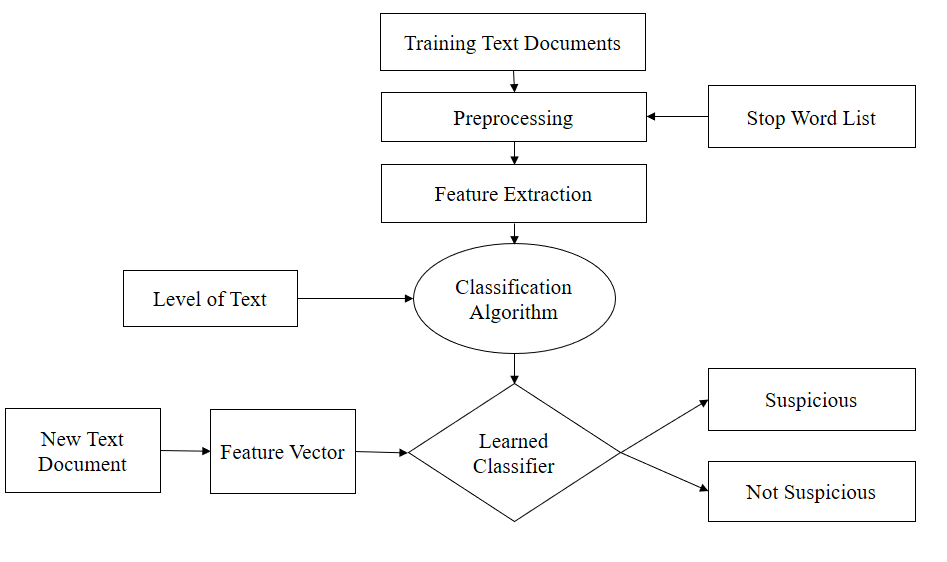
\includegraphics[scale=0.6]{Figures/proposed_model.PNG}
  \caption{Proposed Model of Suspicious Text Detection}
  \label{fig:proposed_model}
\end{figure}
 
 \section{Training Text Corpus}
 Supervised learning involves using a set of training examples that make up the training data. In linguistics, a corpus or text corpus is a large and structured set of texts nowadays usually electronically stored and processed. For a machine learning algorithm a well corpus is essential to perform according to expectation. In the corpus each training example consists of an input text and desired output value. An algorithm is then applied to the data to produce a classifier which will determine the correct output for any further valid input values. In Bengali language processing there is no corpus available which contains suspicious text. But as ours is a supervised classification system, our suspicious text detector needs a training corpus which consist of text and labels indicating whether a text is suspicious or non-suspicious. To implement this system we collect a large amount of Bangla  suspicious text. This texts are collected from online blogs, newspaper, Facebook post and other type of electronic source. Training corpus is divided into positive set (Suspicious text) and negative set (non-suspicious text). The accuracy of the learning algorithms depend on uniqueness of training examples.
 
 \section{Preprocessing}
 In natural language processing, data preprocessing is an essential step. Data preprocessing is a data mining technique that involves transforming raw data into an understandable format. Real world data is often incomplete, inconsistent, and/or lacking in certain behaviors or trends, and is likely to contain many errors. Data preprocessing is a proven method of resolving such issues. Data preprocessing is required to fill in missing values, smooth noisy data, identify or remove the outliers, and resolve inconsistencies.
 Words with no significance must be removed from the text. In our system all texts are preprocessed by the preprocessor. We use main bodies of the text to train suspicious text detector. We are going to represent our text document by list of words and their frequencies. We have a stop word list which consist of words that make no contribution to classify text. In our preprocessing section, such word will be removed by matching with stop word list. It will be very helpful to increase efficiency of the system because redundant will slow our system and increase computational complexity of the system.
 
\section{Feature Extraction}
Word frequencies will be used as feature in our proposed system. Word frequencies are used as features quite often, and although they are usually considered a basic feature, they can prove to be effective.
Terms associated with feature extraction of our system are described shortly.
\subsection{CountVectorizer}

CountVectorizers used to learn the vocabulary of a set of texts and then transform them into a data-frame that can be used for building models. CountVectorizer takes few parameter that is important for extracting feature accurately.

\subparagraph{Stop Words :}
CountVectorizer just counts the occurrences of each word in its vocabulary, extremely common words stop words will become very important features while they add little meaning to the text. In our system we do not take those words into account which improves system accuracy.
\subparagraph{Min-DF, Max-DF :}
These parameters are the minimum and maximum document frequencies words/n-grams must have to be used as features. If either of these parameters are set to integers, they will be used as bounds on the number of documents each feature must be in to be considered as a feature. If either is set to a float, that number will be interpreted as a frequency rather than a numerical limit.
\subparagraph{Max-Features :}
\texttt{max\_features} parameter is used to limit maximum number of feature used by the model. In our system we take most frequent 1000 words by using this parameter to reduce time and storage complexity.

\subsection{Word2vec}
Word2vec is used to train different learning model. Word2vec takes as its input a large corpus of text and produces a vector space, typically of several hundred dimensions, with each unique word in the corpus being assigned a corresponding vector in the space. Word vectors are positioned in the vector space such that words that share common contexts in the corpus are located in close proximity to one another in the space. Accuracy increases overall as the number of words used increases, and as the number of dimensions increases. But we should be careful about associated complexities. 

\subsection{TF-IDF}
The tf–idf is the product of two statistics, term frequency and inverse document frequency. There are various ways for determining the exact values of both statistics.

\subparagraph{Term Frequency}$tf(t,d)$, the simplest choice is to use the raw count of a term in a document, i.e., the number of times that term $t$ and occurs in document $d$.If we denote the raw count by $f_{t,d}$, then the simplest $tf$ scheme is $tf(t,d) = f_{t,d}$. Term frequencies can be calculated in  different ways,
\begin{enumerate}
    \item Term Frequency : 
    \begin{equation}
        \dfrac{f_{t,d}}{\sum_{t'\epsilon d}^{}f_{t',d}}
    \end{equation}
    \item Logarithmically scaled frequency :
    \begin{equation}
         tf(t,d)=\log(1+f_{t,d})
    \end{equation}
   
    \item To prevent bias for longer documents following equation is used:
    \begin{equation}
        tf(t,d) = 0.5 + 0.5 * \frac{f_{t,d}}{\max{(f_{t',d}\colon t'\epsilon d)}}
    \end{equation}
\end{enumerate}

\subparagraph{Inverse Document Frequency}
is a measure whether a term is common or rare across all document. IDF can be calculated by following equation,
\begin{equation}
    idf(t,d) = \log \frac{N}{\abs{1+(d\epsilon D\colon t\epsilon d)}}
\end{equation}
\noindent
%\vspace{0.5cm}
$N$ : Total number of documents in the corpus $N = \abs{D}$\newline
$(d \epsilon D\colon t\epsilon d)$ : \textrm{Number of document where term $t$ appears.}\newline
\vspace{0.5cm}
Now $tf-idf$ is calculated as,
\begin{equation}
    tfidf(t, d, D) = tf(t, d)*idf(t, D)
\end{equation}
So, Final weighting scheme of $tf-idf$ is,
\begin{equation}
        tfidf(t, d, D)=(0.5 + 0.5 * \frac{f_{t,d}}{\max{(f_{t',d}\colon t'\epsilon d)}})*\log \frac{N}{n_t}
\end{equation}
\clearpage

\section{Classification Algorithm}
After extracting feature from the text, now these features are used to train our machine learning model. Different classification algorithms have been used for training purpose.

\subsection{Naive Bayes Classifier}
Naive Bayes is a simple technique for constructing classifiers using feature values. All naive Bayes classifiers assume that the value of a particular feature is independent of the value of any other feature, given the class variable. \textbf{Fig} \ref{fig:NBC} shows decision boundary for Naive Bayes classifier.

\begin{figure}[h!]
    \centering
    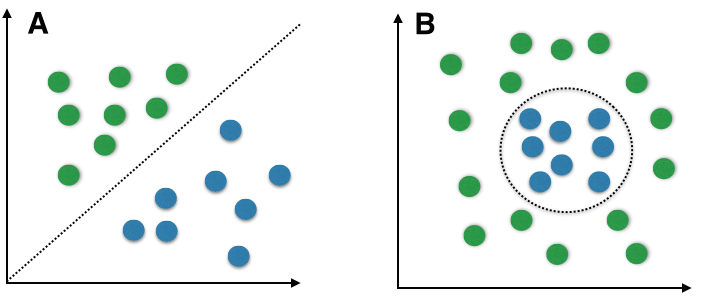
\includegraphics[scale=0.4]{Figures/naive_bayes.png}
    \caption{Naive Bayes Classifier}
    \label{fig:NBC}
\end{figure}

%%% Citation ache %%%%%%
As a popular classification algorithm, Naive Bayes algorithm [4] will be used in our system. It can be defined as Bayes theorem with a conditional independency assumption that all variables $A_{1},A_{2},...,A_{n}$ in a given category $C$ are conditionally independent with each other given $C$. 
According to Bayes rule for a text document $(T)$ and class $(C)$ we can write,$$ P(C|T) = \frac{P(T|C)P(C)}{P(T)}$$
The class we are looking for to assign this document is out of all classes the one that maximizes the probability of that class given the document.
\begin{equation}\label{eq:11}
 \begin{aligned}
     C_{MAP} & = argmax P(C|T) \\     & = argmax \frac{P(T|C)P(C)}{P(T)}\\
    & = argmax {P(T|C)P(C)}
\end{aligned}
\end{equation}
So final equation for Naive Bayes Classifier is,
\begin{equation}
     C_{MAP} = argmax P(X_{1},X_{2},...,X_{n}|C)P(C)
\end{equation}


%%%%%%%%%%% Chapter 4 Implementation %%%%%%%%%%%%%%%
%%%%%%%%%%%%%%%%%%%%%%%%%%%%%%%%%%%%%%%%%%%%%%%%%%%%
%\chapter{Implementation}
\thispagestyle{empty}
The suspicious text detection system implementation consist of different modules. In this chapter we will see the implementation details of this modules. Finally we will see sample input and output of our system.

\section{System Requirements}
Our system takes Bengali text as input and classifies it as suspicious or non-suspicious. To implement this system some hardware and software tools are needed. Required hardware and software tools are listed below.
\subsection{Hardware Requirements}
From input to output the system propagate the following hardware :
\begin{itemize}
    \item Nvidia GeForce GTX 1070 GPU
    \item Minimum GPU RAM 8GB
    \item Physical memory 32GB
    \item Intel core i7-7700K CPU
    \item Solid State Drive (SSD) 256GB
    \item Minimum 2h backup UPS
    \item GPU cooler
    \item Monitors
\end{itemize}
\clearpage
\subsection{Software Requirements}
We implement our system in a specific software environment. Required software lists are,

\begin{itemize}
    \item Operating System : ubuntu 16.04, windows 10
    \item Python 3.0
    \item tensorflow-gpu==1.3.0
    \item djangorestframework==3.7.7
    \item numpy==1.12.1
    \item Django==1.11
    \item Pygments==2.2.0
    \item Markdown==2.6.10
    \item coreapi==2.3.3
    \item psycopg2==2.7.3.2
    \item dj-database-url==0.4.2
    \item gunicorn==19.7.1
    \item whitenoise==3.3.1
    \item django-filter==1.1.0
    \item drf-extensions==0.3.0
    \item spyder 3.6
    \item jupyter notebook
\end{itemize}
\par
\vspace{0.5cm}
\noindent
All of this softwares are not required at a time. To implement different part of our system this softwares were used. To test our system one just need an IDE where the system could be run.

\clearpage
\section{Implementation Details}
We implement the system at different steps from training to testing. These steps are,
\subsection{Training Corpus}
Training corpus is key to suspicious text detection system. No pre-build corpus is available for suspicious Bangla text. We build the corpus and it takes six months to collect data form different online and offline sources. Our training corpus is divided into two folder one is for suspicious and another is for non suspicious text. \textbf{Fig.} \ref{fig:CAP} shows categorical folder of our system.
\begin{figure}[h!]
    \centering
    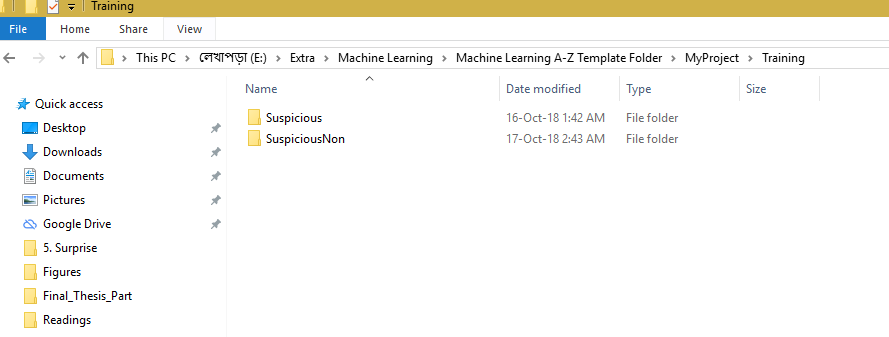
\includegraphics[scale=0.6]{Figures/categorical_fld.PNG}
    \caption{Categorical Folder}
    \label{fig:CAP}
\end{figure}
\par\noindent
\vspace{0.5cm}
\textbf{Fig.}\ref{fig:SMT} shows sample training texts of our system.
\begin{figure}[h!]
    \centering
    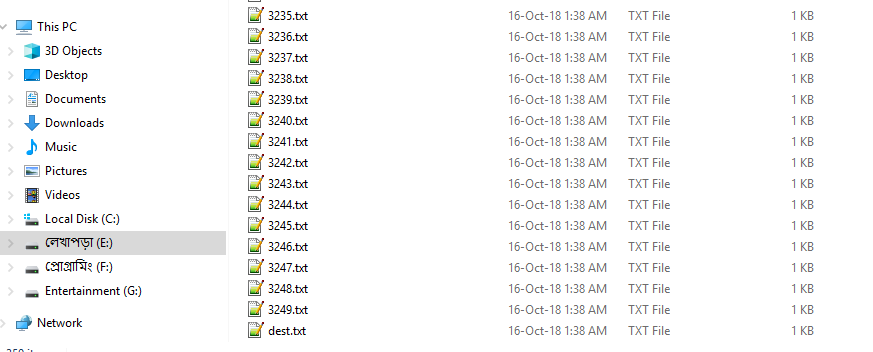
\includegraphics[scale=0.6]{Figures/sample_train.PNG}
    \caption{Sample Training Texts}
    \label{fig:SMT}
\end{figure}

\subsection{Stopword List}
\textbf{Fig.} \ref{fig:stpw} shows a list of some stopword.
In our system the words which has no contribution to classify text is referred as stopwords. From our training text such stopwords were removed. 635 stopwords were collected, from which a list of stopword was built. Removal of this unnecessary words help to increase efficiency of our system.


\begin{figure}[h!]
    \centering
    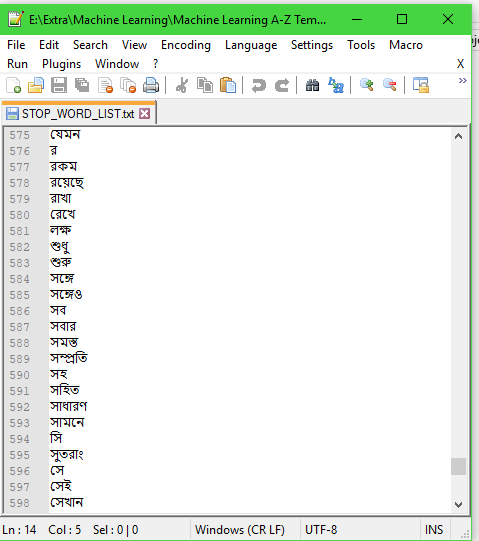
\includegraphics[scale=0.55]{Figures/stp_wrd.PNG}
    \caption{Sample Stopword}
    \label{fig:stpw}
\end{figure}
\par\noindent

\textbf{Fig.} \ref{fig:lstpw} shows the list of stopwords after loading them into our system environment.
\begin{figure}[h!]
    \centering
    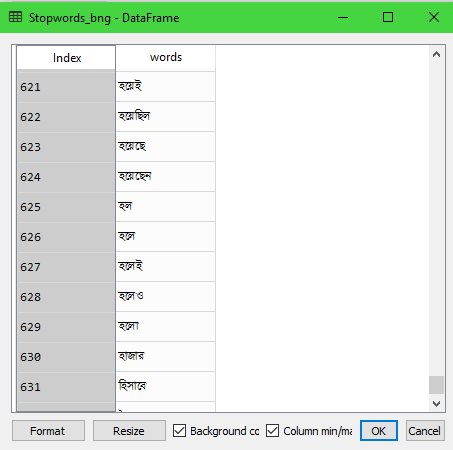
\includegraphics[scale=0.6]{Figures/lstp_wrd.PNG}
    \caption{Stopword in System Environment}
    \label{fig:lstpw}
\end{figure}
\subsection{Processed Corpus}
Processed corpus is the list of all processed text from which we are ready to extract feature. A processed corpus can be created by following steps,
\begin{itemize}
    \item Tokenization of a text.
    \item Punctuation and stopword removal.
    \item Append back remaining words in the text.
\end{itemize}
\textbf{Fig.} \ref{fig:tkn} shows tokenization of a text.
\begin{figure}[h!]
    \centering
    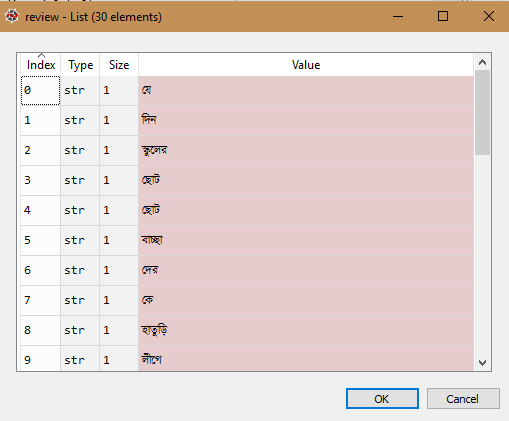
\includegraphics[scale=0.6]{Figures/tokenize.PNG}
    \caption{Tokenized Text}
    \label{fig:tkn}
\end{figure}
\par\noindent
\textbf{Fig.} \ref{fig:crps} shows text corpus in our system environment.
\begin{figure}[h!]
    \centering
    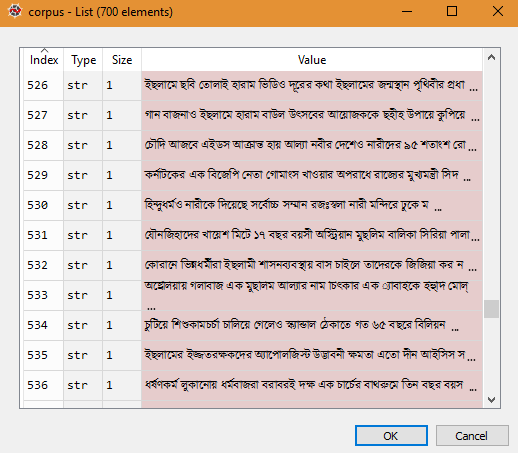
\includegraphics[scale=0.6]{Figures/corpus.PNG}
    \caption{Corpus in System Environment}
    \label{fig:crps}
\end{figure}

\subsection{Corpus Feature}
\textbf{Fig.} \ref{fig:feature} shows a part of our training set feature space.
After processing the texts our next step is to extract feature from the processed text corpus. Feature extraction is an important step because our classifier will learn from the features we extract from texts. More feature will help our classifier model to classify texts more accurately.

\par\noindent
\begin{figure}[h!]
    \centering
    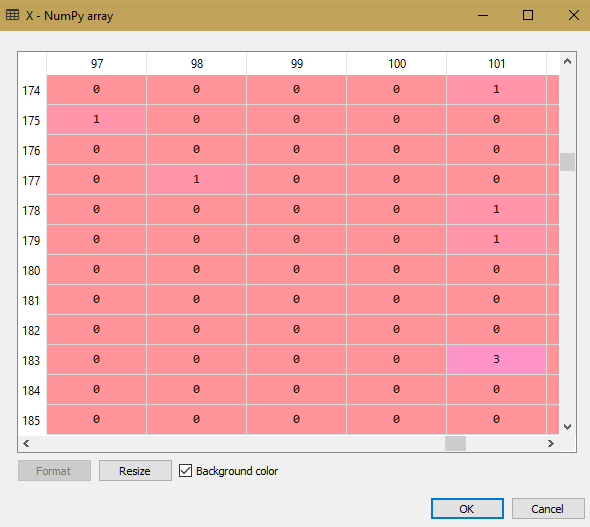
\includegraphics[scale=0.9]{Figures/feature.PNG}
    \caption{Feature Space of Training Set}
    \label{fig:feature}
\end{figure}
\par\noindent
Our feature space is a two dimensional array where rows represents each text of the corpus and columns represents number of unique words available in the corpus. Each cell of the array represents the number of time a specific word occurs in a specific text. 
%\clearpage
\subsection{Labeling of Text}
\textbf{Fig.} \ref{fig:lbt} shows the labeling of texts.
In our system each of the text is labeled with either $0$ or $1$. If the texts are not labeled then the system will not be able to process it. Here $0$ represents suspicious text and $1$ represents non suspicious text. 
\begin{figure}[h!]
    \centering
    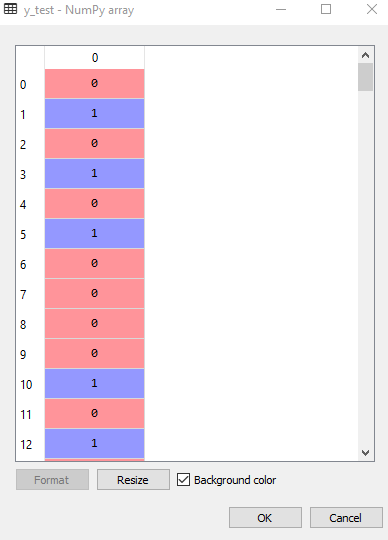
\includegraphics[scale=0.55]{Figures/label_of_text.PNG}
    \caption{Labeling of Texts}
    \label{fig:lbt}
\end{figure}
%\clearpage
\subsection{Prediction of Classifier}
\textbf{Fig.} \ref{fig:prd} shows prediction for a test set.
Our classifier predicts from its learning ability. Each cell of the prediction array represent a prediction for a text. If prediction is $0$ then the text is suspicious otherwise the text is non suspicious.
\begin{figure}[h!]
    \centering
    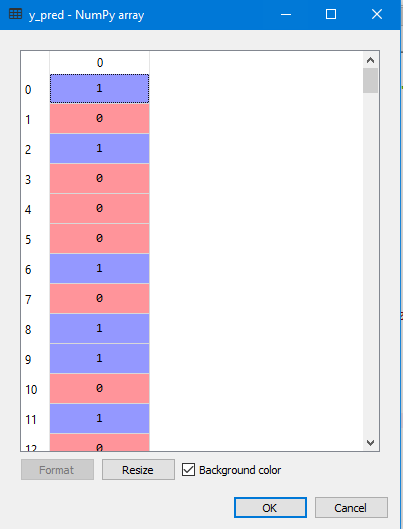
\includegraphics[scale=0.55]{Figures/prediction.PNG}
    \caption{Prediction Array}
    \label{fig:prd}
\end{figure}

\section{Sample Input and Output}
\textbf{Fig.} \ref{fig:smi} shows the inputs of the user in our sample input folder. This is the most important part of our system. We have to check how well our system predict for a sample suspicious and non suspicious text. We will take user inputs in a sample input folder as .txt file. Then this inputs is processed and generate corresponding prediction by our model.\par\vspace{0.5cm}
\begin{figure}[h!]
    \centering
    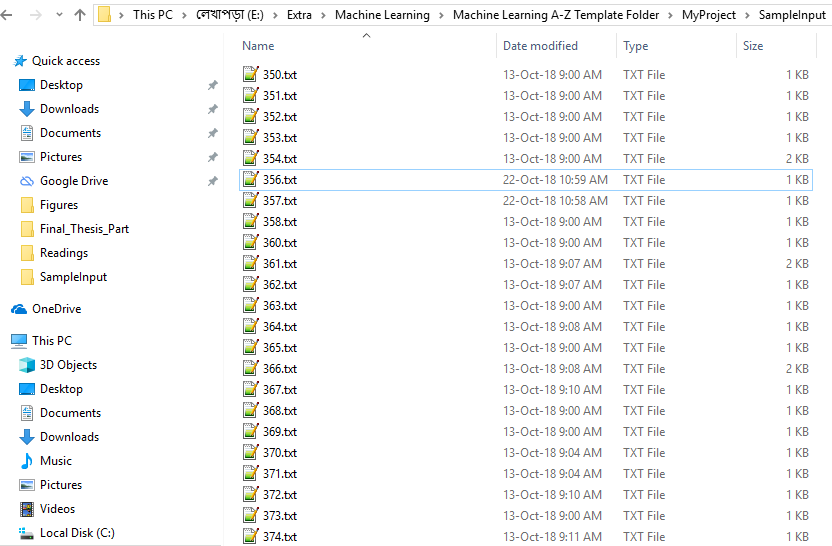
\includegraphics[scale=0.65]{Figures/sample_inp.PNG}
    \caption{Input Folder}
    \label{fig:smi}
\end{figure}
\par\noindent
\vspace{0.3cm}
\textbf{Fig.} \ref{fig:ui} shows a random input of the user.
\begin{figure}[h!]
    \centering
    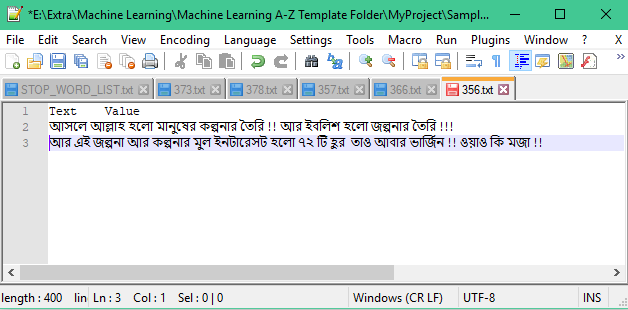
\includegraphics[scale=0.7]{Figures/input_s.PNG}
    \caption{Random Sample Input}
    \label{fig:ui}
\end{figure}
\par\noindent
\textbf{Fig.} \ref{fig:out} shows the prediction of our model. Sample text is user input text and our model predict it as a suspicious or a non suspicious text.
\par
\vspace{1cm}
\begin{figure}[h!]
    \centering
    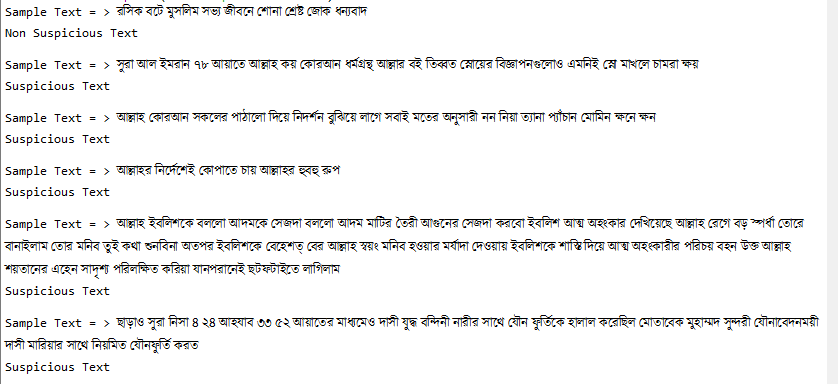
\includegraphics[width=15cm, height=14cm]{Figures/output.PNG}
    \caption{Output in System Environment}
    \label{fig:out}
\end{figure}

%%%%%%%%%% Chapter 5 Experimentation %%%%%%%%%%%%%%
\chapter{Experimentation}
\thispagestyle{empty}
In this chapter we will discuss about our dataset preparation process. We will learn about different evaluation measures. Finally by using this evaluation matrices we will evaluate the result of our system.

\section{Dataset}
Behind the success of any machine learning algorithm dataset is the key. Unfortunately, when we start this project there were no dataset available which can be used in our system. It was a very challenging task for us to build a corpus which contains a large amount of suspicious text. It took us approximately  six month to a build a well furnished  suspicious text corpus containing 4000 suspicious text. We collect non suspicious data from a pre-build corpus[16], thanks to them. At the time of collecting data we were very careful because as a machine leaning model our system learn form what we give to it. If we give wrong data then final output we will not be accurate. \par \vspace{0.5cm}\noindent 
We mark a text as suspicious if it satisfies any one of the following criteria.

\begin{itemize}
    \item Texts contain words which hurts our religious feelings.
    \item Texts which instigate people against government.
    \item Texts which instigate people against law enforcement agencies.
    \item Texts which instigate a community without any reason.
    \item Texts which instigate our political parties. 
    
\end{itemize}
As dataset is collected manually it may have some inconsistency.
\clearpage
\noindent
Most of our suspicious data about religion are collected from online blogs[18-20]. Suspicious data about politics is collected from websites of different newspaper[20,21]. Data is also collected from different pages of Facebook[24]. For some limitation we could not able to use all the data that we collect. Table 5.1 represents the statistics of data used for our model.
\renewcommand{\arraystretch}{1.3}
\begin{table}[h!]
\begin{center}
\caption{Data Summary}
\begin{tabular}{|m{6cm} | m{3cm}|}
\hline
     Number of documents & 700 \\
\hline
     Number of sentences & 3455\\
\hline 
     Number of words & 15547\\
\hline 
     Total unique words & 2954\\
\hline
\end{tabular}
\end{center}
\end{table}
\noindent
In order to classify the texts, we have to feed our collected documents to our classifier model. Table 5.2 shows the summary of dataset used for our classification process.
\renewcommand{\arraystretch}{1.3}
\begin{table}[h!]
\begin{center}
\caption{Data Summary}
\begin{tabular}{|m{6cm} | m{3cm}| m{3cm}|}
\hline
     & Training & Testing \\
\hline
     Number of class & 2 & 2\\
\hline 
     Number of documents & 527 & 173\\
\hline 
     Average word per documents & 23 & 23\\
\hline
\end{tabular}
\end{center}
\end{table}

\section{Evaluation Measures}
In order to evaluate our proposed system, we used several evaluation matrices. We will learn about this  evaluation matrices in this section. Some of this evaluation matrices are,
\begin{itemize}
    \item Confusion Matrix
    \item Precision
    \item Recall
    \item $F_1$ score
    \item Accuracy 
\end{itemize}
Some graphical measures are also used to evaluate our system such as, precision-recall curve, Receiver operating characteristics (ROC) curve.
\clearpage
\subparagraph{Confusion Matrix :}
A confusion matrix is a table that is used to evaluate the performance of a classification model. As ours is a binary classification model, the confusion matrix of our system has two rows and two columns. This matrix reports the number of false positives, false negatives, true positives, and true negatives.

\begin{figure}[h!]
    \centering
    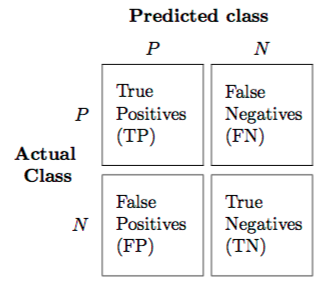
\includegraphics[scale=0.55]{Figures/confusion_matrix_1.png}
    \caption{Confusion Matrix}
    \label{fig:CM}
\end{figure}
\noindent
Above figure shows the confusion matrix. For our system,
\begin{itemize}
    \item True Positive(TP): Number of documents that is suspicious and also classified as suspicious.
    \item True Negative(TN): Number of documents that is non suspicious and also classified as non suspicious.
    \item False Negative(FN): Number of documents that is suspicious but classified as non suspicious.
    \item False Positive(FP): Number of documents that is non suspicious but classified as suspicious. 
\end{itemize}
\noindent
This numbers are used to calculate other evaluation measures.

\subparagraph{Precision :}
Precision referrers as positive predictive value. That is the ratio of
correctly classified positive instances to the total number of instances classified as positive. Precision can be obtained form  the following equation.
\begin{equation}
    \texttt{Precision} = \frac{TP}{TP+FP}
\end{equation}
If precision is high then the algorithm is doing well.

\subparagraph{Recall :}
Recall is the ratio of correctly classified positive instances to the total number of positive instances. It is also called true positive rate. Recall can be obtained from the following equation.
\begin{equation}
    \texttt{Recall} = \frac{TP}{TP+FN}
\end{equation}
High precision and high Recall is essential for a model. Unfortunately there is a trade-off between precision and recall. That is, improving precision typically reduces recall and vice versa. 
\begin{itemize}
    \item If threshold of a classifier is increased then it causes high precision and low recall.
    \item If threshold of a classifier is decreased then it causes low precision and high recall.
\end{itemize}
To sort out this problem we need another measure that is $F_1$measure.

\subparagraph{$F_1$ score :}
 $F_1$ score is the weighted average of Precision and Recall. Therefore, this score takes both false positives and false negatives into account. $F_1$ is usually more useful than accuracy. Accuracy works best if false positives and false negatives have similar cost. If the cost of false positives and false negatives are very different, it’s better to look at both Precision and Recall. F1-score can be obtained from the following equation,
 \begin{equation}
     F_1 = \frac{2*precision*recall}{precision+recall}
 \end{equation}
To chose a learning algorithm between several algorithms we have to find $F_1$ Score of algorithms. The algorithm which has highest $F_1$ score value is chosen as our learning algorithm.

\subparagraph{Accuracy :}
 Accuracy is the most intuitive performance measure and it is simply a ratio of correctly predicted observation to the total observations. For our system accuracy can be obtained by following equation,
\begin{equation}
    \texttt{Accuracy } = \frac{TP+TN}{TP+TN+FP+FN}
\end{equation}

Error of our system can be obtained easily after calculating accuracy,
\begin{equation}
    \texttt{Error} = 1-\texttt{Accuracy}
\end{equation}
We use two graphical measure to evaluate our system. These measures are,
\subparagraph{Precision Recall Curve :}
Precision Recall curves summarize the trade-off between the true positive rate and the positive predictive value for a predictive model using different probability thresholds. A precision-recall curve is a plot of the precision (y-axis) and the recall (x-axis) for different thresholds.

\subparagraph{ROC Curve :}
Receiver Operating Characteristic (ROC) Curves summarize the trade-off between the true positive rate and false positive rate for a predictive model using different probability thresholds. ROC curves are appropriate when the observations are balanced between each class. It is a plot of the false positive rate (x-axis) versus the true positive rate (y-axis) for a number of different candidate threshold values between 0 and 1.

\section{Experimental Results}
Table 5.3 represents Accuracy and Error rate of different classification algorithm on our dataset.
\renewcommand{\arraystretch}{1.5}
\begin{table}[h!]
\begin{center}
\caption{Evaluation Summary}
\begin{tabular}{|m{7cm} | m{3cm}| m{3cm}|}
\hline
     & Accuracy (\%) & Error (\%) \\
\hline
    Naive Bayes & 0.85 & 0.15\\
\hline 
    SVM (Linaer Kernel) & 0.91 & 0.09\\
\hline 
    SVM (RBF Kernel) & 0.90 & 0.10\\
\hline 
    Logistic Regression & 0.92 & 0.08\\
\hline
    K-Nearest Neighbor & 0.73 & 0.27\\
\hline
    Decision Tree & 0.88 & 0.12\\
\hline
\end{tabular}
\end{center}
\end{table}
\par
\noindent
From the evaluation summary we can see that Logistic Regression and Support Vector Machine algorithm's are performing up to the mark on our dataset . Naive Bayes and Decision tree also doing really well. But accuracy of K-nearest neighbour is really poor compare to other algorithms. 
\clearpage
\noindent
Table 5.4 shows the precision, recall and $F_1$ score of different classification algorithm used in our model.

\begin{table}[h!]
\begin{center}
\caption{Comparison of Results}
\begin{tabular}{|m{6.8cm} | m{2cm}| m{2cm}| m{2cm}|}
\hline
     & Precision & Recall & $F_1$ score \\
\hline
    Naive Bayes & 0.89 & 0.85 & 0.85\\
\hline 
    SVM (Linaer Kernel) & 0.91 & 0.91 & 0.91\\
\hline 
    SVM (RBF Kernel) & 0.90 & 0.91 & 0.90\\
\hline 
    Logistic Regression & 0.91 & 0.93 & 0.93\\
\hline
    K-Nearest Neighbor & 0.82 & 0.73 & 0.70\\
\hline
    Decision Tree & 0.88 & 0.92 & 0.89\\
\hline
\end{tabular}
\end{center}
\end{table}
\noindent
For all of the algorithms we use similar number of test documents. Logistic Regression performs well than other algorithm.
\par
\vspace{0.5cm}
\noindent
Table 5.4 shows comparison among six algorithms algorithms that were used in our system successfully. The $F_1$ score of Naive Bayes algorithm is 0.85 which is quite well. The result of SVM with linear kernel is quite similar as SVM with RBF kernel. But Linear kernel has better $F_1$ score than RBF kernel. Logistic Regression outperform all other algorithm, it has $F_1$ score of 0.93. Decision tree also performs well but $F_1$ score of K-nearest neighbor is the lowest.

\par
\vspace{0.5cm}
\noindent
Now, we will learn about classification report, Precision Recall curve and Receiver operating characteristic's (ROC) curve of  all of this algorithms. Classification report gives us precision, recall and $F_1$ score of each category which is really helpful to analyze the algorithm. From classification report we can see what category our model can can more accurately and what should we do to increase the accuracy of the system. Precision Recall curve and ROC curve shows the graphical evaluation of algorithms. Precision Recall curve shows value of precision and recall at different threshold values. ROC curve shows relation between true positive rate and false positive rate. 
\clearpage

%%%%%%%%% Naive Bayes Classifier %%%%%%%%%%%
%%%%%%%%%%%%%%%%%%%%%%%%%%%%%%%%%%%%%%
\subsection{Result of Naive Bayes Classifier}
Table 5.5 shows the classification report for Naive Bayes classifier. Here support expose the total number of document test by the system.

\begin{table}[h!]
\begin{center}
\caption{Classification Report (Naive Bayes)}
\begin{tabular}{|m{4.4cm} | m{2cm}| m{2cm}| m{2cm}| m{2cm}|}
\hline
     & Precision & Recall & $F_1$ score & Support \\
\hline
     Suspicious & 1.00 & 0.71 & 0.83 & 89\\
\hline 
     Non suspicious  & 0.76 & 1.00 & 0.87 & 84\\
\hline 
     avg./total & 0.89 & 0.85 & 0.85 & 173\\
\hline
\end{tabular}
\end{center}
\end{table}

\noindent
\textbf{Fig.} \ref{fig:prn} shows precision recall curve for Naive Bayes classifier.

\begin{figure}[h!]
    \centering
    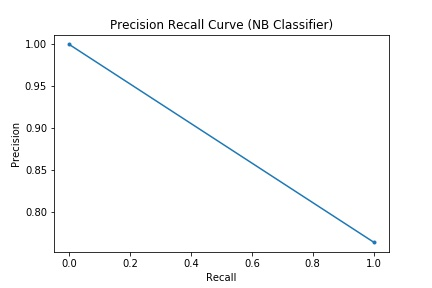
\includegraphics[scale=0.58]{Figures/PRN.jpg}
    \caption{Precision Recall Curve (Naive Bayes)}
    \label{fig:prn}
\end{figure}

\noindent
\textbf{Fig.} \ref{fig:rocn} shows ROC curve for Naive Bayes classifier.

\begin{figure}[h!]
    \centering
    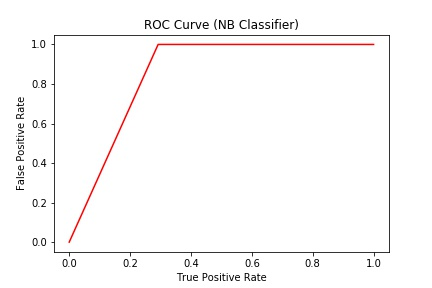
\includegraphics[scale=0.58]{Figures/ROCN.jpg}
    \caption{ROC Curve (Naive Bayes)}
    \label{fig:rocn}
\end{figure}

%%%%%%%%% SVM Linear kernel%%%%%%%%%%%
%%%%%%%%%%%%%%%%%%%%%%%%%%%%%%%%%%%%%%

\subsection{Result of SVM (Linear Kernel)}
Table 5.6 shows the classification report for Support Vector Machine with linear kernel.

\begin{table}[h!]
\begin{center}
\caption{Classification Report (SVM Linear Kernel)}
\begin{tabular}{|m{4.4cm} | m{2cm}| m{2cm}| m{2cm}| m{2cm}|}
\hline
     & Precision & Recall & $F_1$ score & Support \\
\hline
     Suspicious & 0.91 & 1.00 & 0.91 & 89\\
\hline 
     Non suspicious  & 1.00 & 0.90 & 0.91 & 84\\
\hline 
     avg./total & 0.91 & 0.91 & 0.91 & 173\\
\hline
\end{tabular}
\end{center}
\end{table}

\noindent
\textbf{Fig.} \ref{fig:prsl} shows precision recall curve for SVM (Linear Kernel).

\begin{figure}[h!]
    \centering
    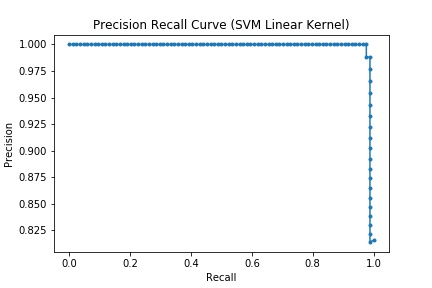
\includegraphics[scale=0.58]{Figures/PRSL.jpg}
    \caption{Precision Recall Curve (SVM Liner Kernel)}
    \label{fig:prsl}
\end{figure}

\noindent
\textbf{Fig.} \ref{fig:rocsl} shows ROC curve for SVM (Linear Kernel).

\begin{figure}[h!]
    \centering
    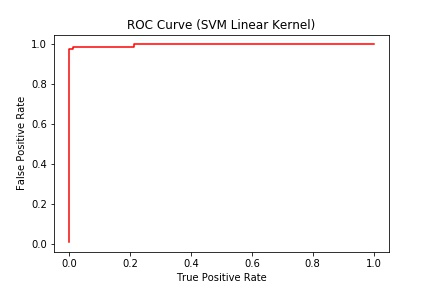
\includegraphics[scale=0.58]{Figures/ROCSL.jpg}
    \caption{ROC Curve (SVM Linear Kernel)}
    \label{fig:rocsl}
\end{figure}

%%%%%%%%% SVM RBF kernel%%%%%%%%%%%
%%%%%%%%%%%%%%%%%%%%%%%%%%%%%%%%%%

\subsection{Result of SVM (RBF Kernel)}
Table 5.7 shows the classification report for Support Vector Machine with RBF or Gaussian kernel.

\begin{table}[h!]
\begin{center}
\caption{Classification Report (SVM RBF Kernel)}
\begin{tabular}{|m{4.4cm} | m{2cm}| m{2cm}| m{2cm}| m{2cm}|}
\hline
     & Precision & Recall & $F_1$ score & Support \\
\hline
     Suspicious & 0.90 & 0.99 & 0.90 & 89\\
\hline 
     Non suspicious  & 0.99 & 0.89 & 0.91 & 84\\
\hline 
     avg./total & 0.90 & 0.91 & 0.90 & 173\\
\hline
\end{tabular}
\end{center}
\end{table}

\noindent
\textbf{Fig.} \ref{fig:prsk} shows precision recall curve for SVM (RBF Kernel).

\begin{figure}[h!]
    \centering
    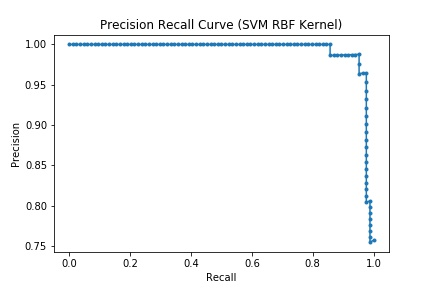
\includegraphics[scale=0.58]{Figures/PRSK.jpg}
    \caption{Precision Recall Curve (SVM RBF Kernel)}
    \label{fig:prsk}
\end{figure}

\noindent
\textbf{Fig.} \ref{fig:rocsk} shows ROC curve for SVM (RBF Kernel).

\begin{figure}[h!]
    \centering
    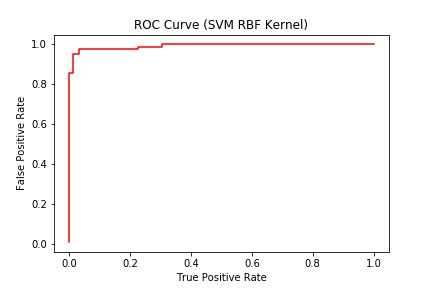
\includegraphics[scale=0.58]{Figures/ROCSK.jpg}
    \caption{ROC Curve (SVM RBF Kernel)}
    \label{fig:rocsk}
\end{figure}

%%%%%%% Logistic Regression %%%%%%%
%%%%%%%%%%%%%%%%%%%%%%%%%%%%%%%%%%%

\subsection{Result of Logistic Regression}
Table 5.8 shows the classification report for Logistic Regression.

\begin{table}[h!]
\begin{center}
\caption{Classification Report (Logistic Regression)}
\begin{tabular}{|m{4.4cm} | m{2cm}| m{2cm}| m{2cm}| m{2cm}|}
\hline
     & Precision & Recall & $F_1$ score & Support \\
\hline
     Suspicious & 0.92 & 1.00 & 0.93 & 89\\
\hline 
     Non suspicious  & 1.00 & 0.93 & 0.93 & 84\\
\hline 
     avg./total & 0.91 & 0.93 & 0.93 & 173\\
\hline
\end{tabular}
\end{center}
\end{table}

\noindent
\textbf{Fig.} \ref{fig:prl} shows precision recall curve for Logistic Regression.

\begin{figure}[h!]
    \centering
    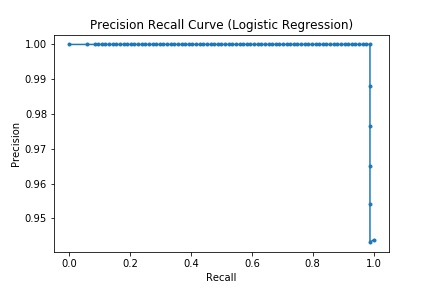
\includegraphics[scale=0.58]{Figures/PRL.jpg}
    \caption{Precision Recall Curve (Logistic Regression)}
    \label{fig:prl}
\end{figure}

\noindent
\textbf{Fig.} \ref{fig:rocl} shows ROC curve for Logistic Regression.

\begin{figure}[h!]
    \centering
    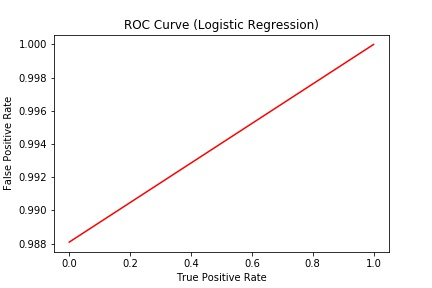
\includegraphics[scale=0.58]{Figures/ROCL.jpg}
    \caption{ROC Curve (Logistic Regression)}
    \label{fig:rocl}
\end{figure}

%%%%%%%% K-Nearest Neighbor %%%%%
%%%%%%%%%%%%%%%%%%%%%%%%%%%%%%%%%

\subsection{Result of K-Nearest Neighbor}
Table 5.9 shows the classification report for K-Nearest Neighbor.

\begin{table}[h!]
\begin{center}
\caption{Classification Report (K-Nearest Neighbor)}
\begin{tabular}{|m{4.4cm} | m{2cm}| m{2cm}| m{2cm}| m{2cm}|}
\hline
     & Precision & Recall & $F_1$ score & Support \\
\hline
     Suspicious & 0.65 & 1.00 & 0.79 & 89\\
\hline 
     Non suspicious  & 1.00 & 0.44 & 0.61 & 84\\
\hline 
     avg./total & 0.82 & 0.73 & 0.70 & 173\\
\hline
\end{tabular}
\end{center}
\end{table}

\noindent
\textbf{Fig.} \ref{fig:prknn} shows precision recall curve for K-Nearest Neighbor.

\begin{figure}[h!]
    \centering
    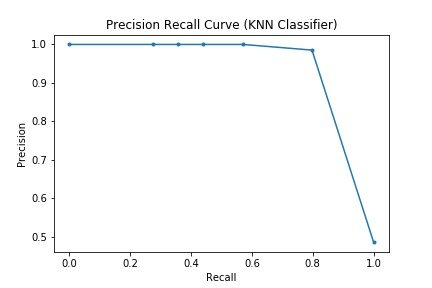
\includegraphics[scale=0.58]{Figures/PRKNN.jpg}
    \caption{Precision Recall Curve (K-Nearest Neighbor)}
    \label{fig:prknn}
\end{figure}

\noindent
\textbf{Fig.} \ref{fig:rocknn} shows ROC curve for K-Nearest Neighbor.

\begin{figure}[h!]
    \centering
    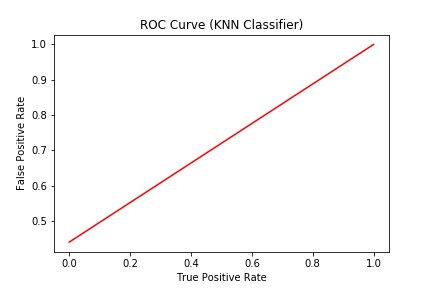
\includegraphics[scale=0.58]{Figures/ROCKNN.jpg}
    \caption{ROC Curve (K-Nearest Neighbor)}
    \label{fig:rocknn}
\end{figure}

%%%%%%%%%%%% Decision Tree %%%%%%%%%%%%
%%%%%%%%%%%%%%%%%%%%%%%%%%%%%%%%%%%%%%%
\subsection{Result of Decision Tree}
Table 5.10 shows the classification report for Decision Tree.

\begin{table}[h!]
\begin{center}
\caption{Classification Report (Decision Tree)}
\begin{tabular}{|m{4.4cm} | m{2cm}| m{2cm}| m{2cm}| m{2cm}|}
\hline
     & Precision & Recall & $F_1$ score & Support \\
\hline
     Suspicious & 0.91 & 0.89 & 0.90 & 89\\
\hline 
     Non suspicious  & 0.88 & 0.90 & 0.89 & 84\\
\hline 
     avg./total & 0.90 & 0.90 & 0.90 & 173\\
\hline
\end{tabular}
\end{center}
\end{table}

\noindent
\textbf{Fig.} \ref{fig:prdct} shows precision recall curve for Decision Tree.

\begin{figure}[h!]
    \centering
    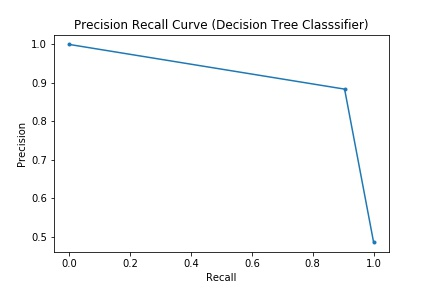
\includegraphics[scale=0.58]{Figures/PRDCT.jpg}
    \caption{Precision Recall Curve (Decision Tree)}
    \label{fig:prdct}
\end{figure}

\noindent
\textbf{Fig.} \ref{fig:rocdct} shows ROC curve for Decision Tree.

\begin{figure}[h!]
    \centering
    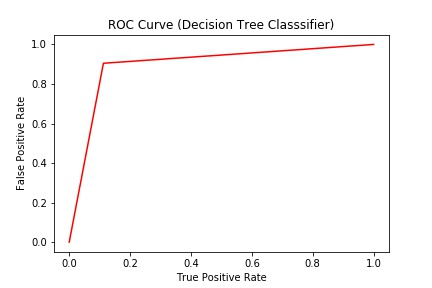
\includegraphics[scale=0.58]{Figures/ROCDCT.jpg}
    \caption{ROC Curve (Decision Tree)}
    \label{fig:rocdct}
\end{figure}

\section{Discussion}


\end{document}

 







